\documentclass[border=5pt, tikz]{standalone}

\usetikzlibrary{
    positioning, arrows.meta, calc, backgrounds,
    decorations.markings, decorations.pathmorphing,
    fit, shapes.geometric, patterns, matrix,
    shadows.blur, fadings
}

\usepackage{amsmath, amssymb, bm}
\usepackage{xcolor}

% ============================================
% MODERN PALETTE (Publication Quality)
% ============================================
\definecolor{primary}{HTML}{2563EB}      % Blue
\definecolor{secondary}{HTML}{7C3AED}    % Purple
\definecolor{accent}{HTML}{F59E0B}       % Amber
\definecolor{success}{HTML}{10B981}      % Green
\definecolor{danger}{HTML}{EF4444}       % Red
\definecolor{neutral}{HTML}{6B7280}      % Gray

\definecolor{bg}{HTML}{FAFBFC}
\definecolor{bgdark}{HTML}{F1F5F9}
\definecolor{border}{HTML}{E2E8F0}
\definecolor{text}{HTML}{1E293B}
\definecolor{textsub}{HTML}{64748B}

% Semantic colors
\definecolor{receiver}{HTML}{DC2626}     % Red for receiver
\definecolor{neighbor}{HTML}{0891B2}     % Cyan for neighbors
\definecolor{hlca}{HTML}{059669}         % Emerald for HLCA
\definecolor{luca}{HTML}{7C3AED}         % Purple for LuCA
\definecolor{context}{HTML}{2563EB}      % Blue for context
\definecolor{drift}{HTML}{F59E0B}        % Amber for drift
\definecolor{flow}{HTML}{EC4899}         % Pink for flow

% ============================================
% PROFESSIONAL STYLES
% ============================================
\tikzset{
    % Cell styles
    cell/.style={
        circle, minimum size=4mm,
        fill=#1!70, draw=#1!90, line width=0.5pt,
        blur shadow={shadow blur steps=5, shadow xshift=0.3mm, shadow yshift=-0.3mm}
    },
    cellsm/.style={circle, minimum size=3mm, fill=#1!60, draw=#1!80, line width=0.4pt},
    receiver cell/.style={
        circle, minimum size=6mm,
        fill=receiver!80, draw=receiver!90, line width=0.8pt,
        blur shadow={shadow blur steps=8, shadow xshift=0.5mm, shadow yshift=-0.5mm}
    },
    % Module styles
    module/.style={
        rectangle, rounded corners=3pt,
        minimum height=8mm, minimum width=20mm,
        fill=#1!15, draw=#1!60, line width=0.6pt,
        font=\fontsize{8}{9}\selectfont\sffamily,
        blur shadow={shadow blur steps=5, shadow xshift=0.3mm, shadow yshift=-0.3mm}
    },
    modulelg/.style={
        rectangle, rounded corners=4pt,
        minimum height=10mm, minimum width=28mm,
        fill=#1!12, draw=#1!50, line width=0.7pt,
        font=\fontsize{9}{10}\selectfont\sffamily\bfseries,
        blur shadow={shadow blur steps=6, shadow xshift=0.4mm, shadow yshift=-0.4mm}
    },
    % Container styles
    panel/.style={
        rectangle, rounded corners=6pt,
        fill=white, draw=border, line width=0.6pt,
        blur shadow={shadow blur steps=8, shadow xshift=0.5mm, shadow yshift=-0.5mm, shadow opacity=0.15}
    },
    subpanel/.style={
        rectangle, rounded corners=4pt,
        fill=bgdark, draw=border!70, line width=0.4pt
    },
    % Arrow styles
    flow/.style={
        -{Stealth[length=2.5mm, width=1.8mm]},
        line width=0.7pt, draw=#1
    },
    flowthick/.style={
        -{Stealth[length=3mm, width=2mm]},
        line width=1pt, draw=#1
    },
    flowdashed/.style={
        -{Stealth[length=2.5mm, width=1.8mm]},
        line width=0.7pt, draw=#1, dashed
    },
    % Label styles
    heading/.style={font=\fontsize{11}{12}\selectfont\bfseries\sffamily, text=text},
    subheading/.style={font=\fontsize{9}{10}\selectfont\sffamily, text=textsub},
    label/.style={font=\fontsize{7}{8}\selectfont\sffamily, text=textsub},
    mathlabel/.style={font=\fontsize{8}{9}\selectfont, text=text},
    dim/.style={
        rectangle, rounded corners=2pt,
        fill=#1!10, draw=#1!40, line width=0.3pt,
        font=\fontsize{7}{8}\selectfont\sffamily,
        inner sep=2pt
    },
    % Equation box
    eqbox/.style={
        rectangle, rounded corners=3pt,
        fill=bgdark, draw=border, line width=0.4pt,
        inner sep=4pt, font=\fontsize{8}{9}\selectfont
    },
}

\begin{document}

% ============================================
% MAIN ARCHITECTURE DIAGRAM
% ============================================
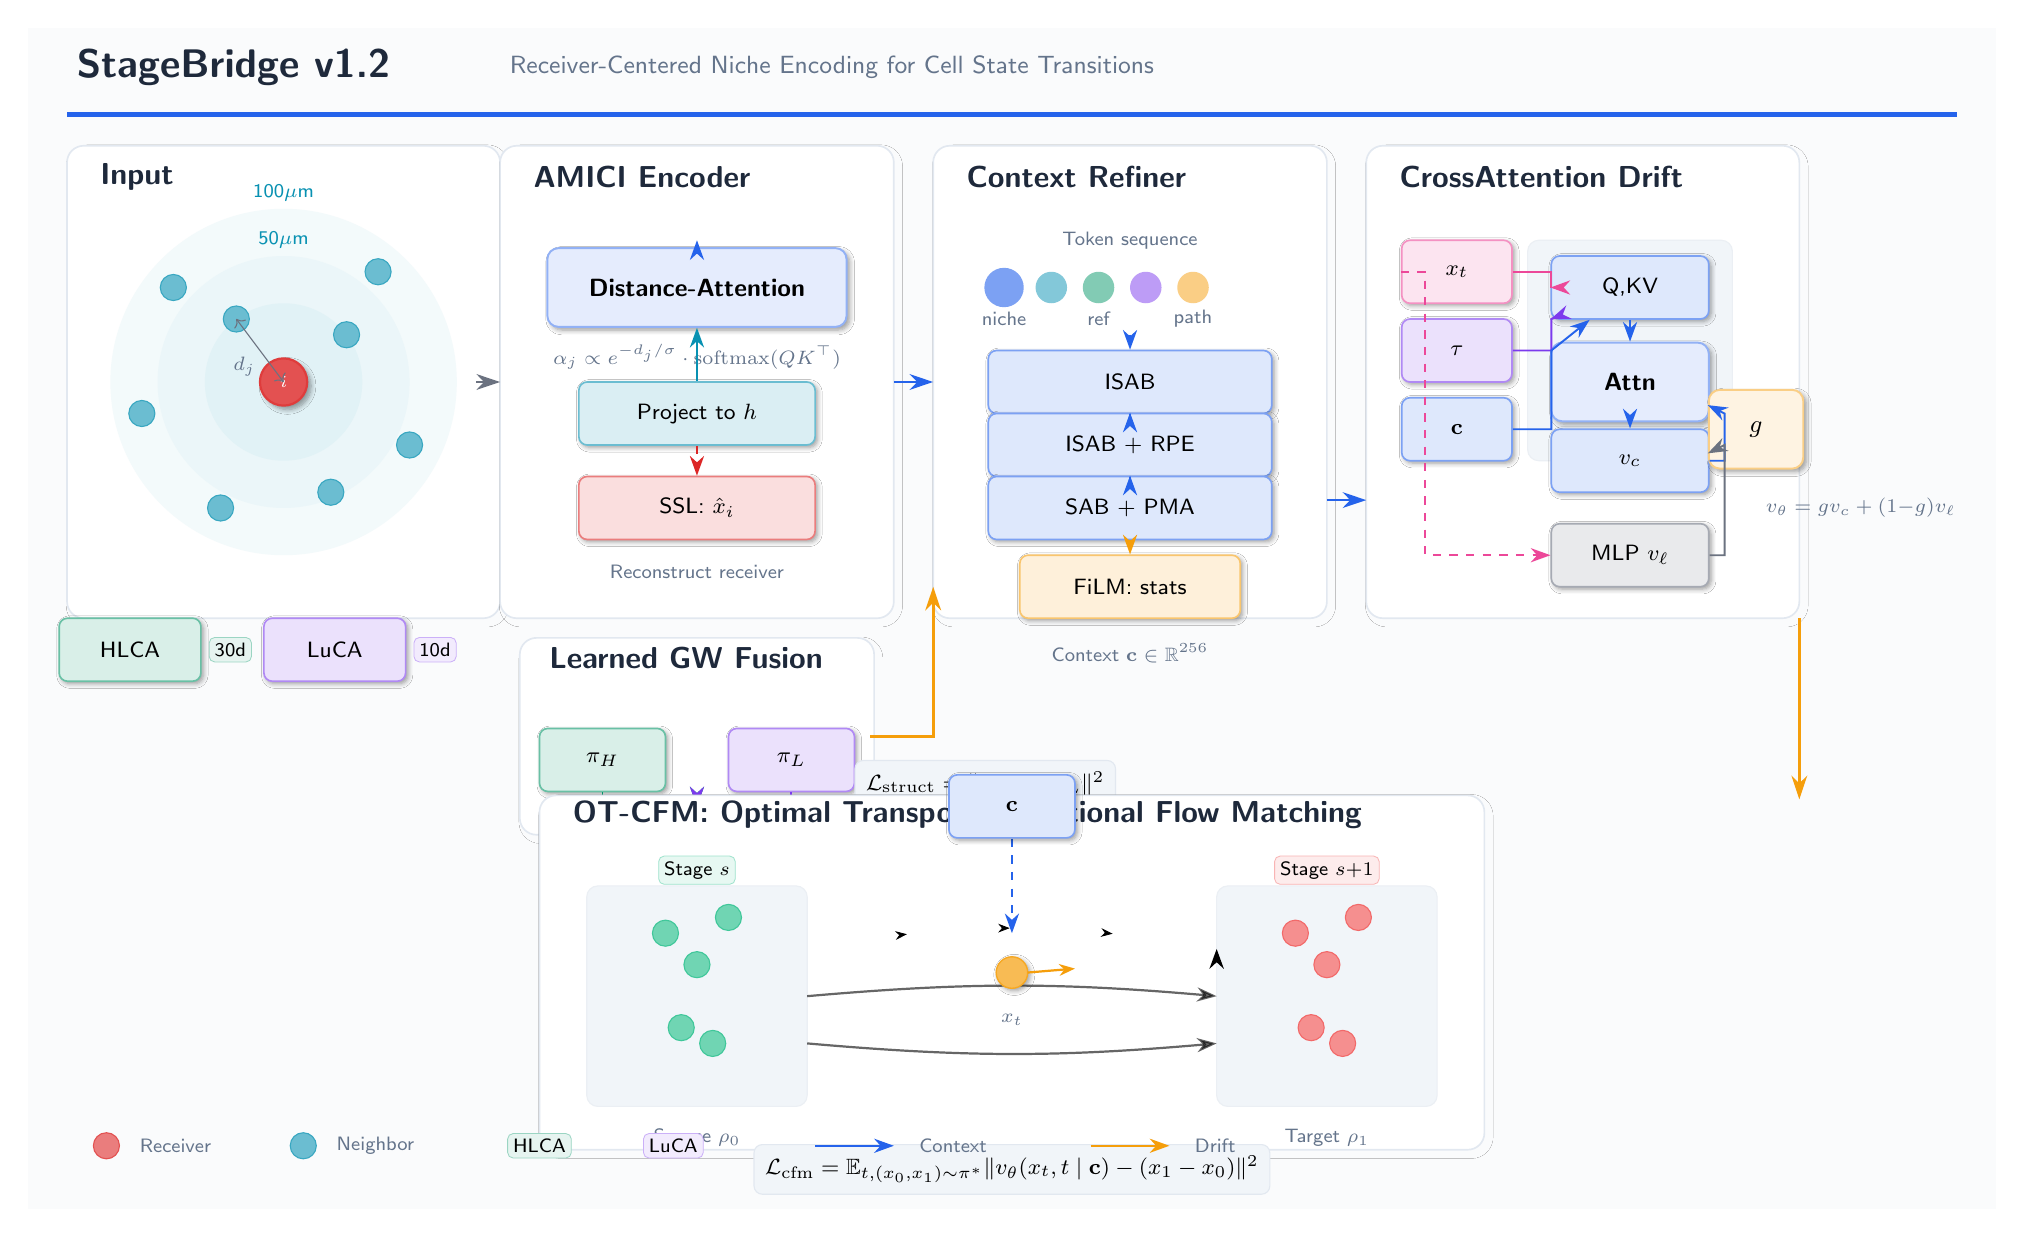
\begin{tikzpicture}[x=1mm, y=1mm]

% Background
\fill[bg] (-5, -5) rectangle (245, 145);

% ============================================
% HEADER
% ============================================
\node[font=\fontsize{14}{15}\selectfont\bfseries\sffamily, text=text, anchor=west]
    at (0, 140) {StageBridge v1.2};
\node[font=\fontsize{9}{10}\selectfont\sffamily, text=textsub, anchor=west]
    at (55, 140) {Receiver-Centered Niche Encoding for Cell State Transitions};
\draw[primary, line width=2pt] (0, 134) -- (240, 134);

% ============================================
% 1. INPUT PANEL (LEFT)
% ============================================
\node[panel, minimum width=55mm, minimum height=60mm] at (27.5, 100) {};
\node[heading, anchor=west] at (3, 126) {Input};

% Spatial Niche visualization
\begin{scope}[shift={(27.5, 100)}]
    % Distance rings
    \fill[neighbor!5] (0,0) circle (22mm);
    \fill[neighbor!8] (0,0) circle (16mm);
    \fill[neighbor!12] (0,0) circle (10mm);

    % Ring labels
    \node[label, neighbor] at (0, 24) {100$\mu$m};
    \node[label, neighbor] at (0, 18) {50$\mu$m};

    % Neighbor cells (sorted by distance)
    \node[cellsm=neighbor] at (-14, 12) {};
    \node[cellsm=neighbor] at (12, 14) {};
    \node[cellsm=neighbor] at (-18, -4) {};
    \node[cellsm=neighbor] at (16, -8) {};
    \node[cellsm=neighbor] at (-8, -16) {};
    \node[cellsm=neighbor] at (6, -14) {};
    \node[cellsm=neighbor] at (-6, 8) {};
    \node[cellsm=neighbor] at (8, 6) {};

    % Receiver cell (center)
    \node[receiver cell] (recv) at (0, 0) {};
    \node[font=\fontsize{6}{7}\selectfont\sffamily, text=white] at (0, 0) {$i$};

    % Distance annotation
    \draw[neutral, line width=0.4pt, <->] (0, 0) -- (-6, 8);
    \node[label] at (-5, 2) {$d_j$};
\end{scope}

% HLCA/LuCA tokens
\begin{scope}[shift={(8, 66)}]
    \node[module=hlca, minimum width=18mm] at (0, 0) {HLCA};
    \node[dim=hlca, anchor=west] at (10, 0) {30d};

    \node[module=luca, minimum width=18mm] at (26, 0) {LuCA};
    \node[dim=luca, anchor=west] at (36, 0) {10d};
\end{scope}

% ============================================
% 2. AMICI ENCODER PANEL
% ============================================
\node[panel, minimum width=50mm, minimum height=60mm] at (80, 100) {};
\node[heading, anchor=west] at (58, 126) {AMICI Encoder};

\begin{scope}[shift={(80, 100)}]
    % Encoder components
    \node[modulelg=context, minimum width=38mm] (attn) at (0, 12) {Distance-Attention};
    \node[label, anchor=north] at (0, 6) {$\alpha_j \propto e^{-d_j/\sigma} \cdot \mathrm{softmax}(QK^\top)$};

    % Input projection
    \node[module=neighbor, minimum width=30mm] (proj) at (0, -4) {Project to $h$};

    % SSL reconstruction
    \node[module=receiver, minimum width=30mm] (ssl) at (0, -16) {SSL: $\hat{x}_i$};
    \node[label, anchor=north] at (0, -22) {Reconstruct receiver};

    % Arrows
    \draw[flow=neighbor] (proj) -- (attn);
    \draw[flow=context] (attn) -- ++(0, 6);
    \draw[flowdashed=receiver] (proj) -- (ssl);
\end{scope}

% Arrow from input to AMICI
\draw[flowthick=neutral] (52, 100) -- (55, 100);

% ============================================
% 3. LEARNED GW FUSION
% ============================================
\node[panel, minimum width=45mm, minimum height=25mm] at (80, 55) {};
\node[heading, anchor=west] at (60, 65) {Learned GW Fusion};

\begin{scope}[shift={(80, 52)}]
    % HLCA projection
    \node[module=hlca, minimum width=16mm] (hproj) at (-12, 0) {$\pi_H$};
    % LuCA projection
    \node[module=luca, minimum width=16mm] (lproj) at (12, 0) {$\pi_L$};
    % Fusion
    \node[module=accent, minimum width=30mm] (fuse) at (0, -10) {Fuse: $[\alpha h + (1{-}\alpha)l; h{-}l]$};

    % Arrows
    \draw[flow=hlca] (hproj) -- ++(0, -5) -| (fuse);
    \draw[flow=luca] (lproj) -- ++(0, -5) -| (fuse);

    % Structure loss annotation
    \node[eqbox, anchor=west] at (20, -3) {\footnotesize $\mathcal{L}_{\mathrm{struct}} = \|D_H - D_L\|^2$};
\end{scope}

% ============================================
% 4. CONTEXT REFINER PANEL
% ============================================
\node[panel, minimum width=50mm, minimum height=60mm] at (135, 100) {};
\node[heading, anchor=west] at (113, 126) {Context Refiner};

\begin{scope}[shift={(135, 100)}]
    % Token sequence
    \node[label] at (0, 18) {Token sequence};

    % Tokens visualization
    \fill[context!60] (-16, 12) circle (2.5mm);
    \fill[neighbor!50] (-10, 12) circle (2mm);
    \fill[hlca!50] (-4, 12) circle (2mm);
    \fill[luca!50] (2, 12) circle (2mm);
    \fill[accent!50] (8, 12) circle (2mm);

    \node[label] at (-16, 8) {niche};
    \node[label] at (-4, 8) {ref};
    \node[label] at (8, 8) {path};

    % Hierarchical Set Transformer
    \node[module=context, minimum width=36mm] (isab1) at (0, 0) {ISAB};
    \node[module=context, minimum width=36mm] (isab2) at (0, -8) {ISAB + RPE};
    \node[module=context, minimum width=36mm] (sab) at (0, -16) {SAB + PMA};

    \draw[flow=context] (0, 6) -- (isab1);
    \draw[flow=context] (isab1) -- (isab2);
    \draw[flow=context] (isab2) -- (sab);

    % FiLM conditioning
    \node[module=accent, minimum width=28mm] (film) at (0, -26) {FiLM: stats};
    \draw[flow=accent] (sab) -- (film);

    \node[label, anchor=north] at (0, -32) {Context $\mathbf{c} \in \mathbb{R}^{256}$};
\end{scope}

% Arrows between panels
\draw[flowthick=context] (105, 100) -- (110, 100);
\draw[flowthick=accent] (102, 55) -- (110, 55) -- (110, 74);

% ============================================
% 5. DRIFT HEAD PANEL
% ============================================
\node[panel, minimum width=55mm, minimum height=60mm] at (192.5, 100) {};
\node[heading, anchor=west] at (168, 126) {CrossAttention Drift};

\begin{scope}[shift={(192.5, 100)}]
    % Inputs
    \node[module=flow, minimum width=14mm] (xt) at (-16, 14) {$x_t$};
    \node[module=secondary, minimum width=14mm] (time) at (-16, 4) {$\tau$};
    \node[module=context, minimum width=14mm] (ctx) at (-16, -6) {$\mathbf{c}$};

    % Context path (cross-attention)
    \node[subpanel, minimum width=26mm, minimum height=28mm] at (6, 4) {};
    \node[module=context, minimum width=20mm] (qkv) at (6, 12) {Q,KV};
    \node[modulelg=context, minimum width=20mm] (attn) at (6, 0) {Attn};
    \node[module=context, minimum width=20mm] (vc) at (6, -10) {$v_c$};

    \draw[flow=flow] (xt) -- (-4, 14) -- (-4, 12) -- (qkv);
    \draw[flow=secondary] (time) -- (-4, 4) -- (-4, 8) -- (qkv);
    \draw[flow=context] (ctx) -- (-4, -6) -- (-4, 4) -- (qkv);
    \draw[flow=context] (qkv) -- (attn);
    \draw[flow=context] (attn) -- (vc);

    % Latent path (MLP)
    \node[module=neutral, minimum width=20mm] (mlp) at (6, -22) {MLP $v_\ell$};
    \draw[flowdashed=flow] (xt) -- (-20, 14) -- (-20, -22) -- (mlp);

    % Gate
    \node[modulelg=drift, minimum width=12mm] (gate) at (22, -6) {$g$};
    \draw[flow=context] (vc) -- (18, -10) -- (18, -4) -- (gate);
    \draw[flow=neutral] (mlp) -- (18, -22) -- (18, -8) -- (gate);

    % Output
    \node[label, anchor=west] at (22, -16) {$v_\theta = gv_c + (1{-}g)v_\ell$};
\end{scope}

% Arrow from context refiner
\draw[flowthick=context] (160, 85) -- (165, 85);

% ============================================
% 6. OT-CFM PANEL (BOTTOM)
% ============================================
\node[panel, minimum width=120mm, minimum height=45mm] at (120, 25) {};
\node[heading, anchor=west] at (63, 45) {OT-CFM: Optimal Transport Conditional Flow Matching};

\begin{scope}[shift={(120, 22)}]
    % Source distribution
    \node[subpanel, minimum width=28mm, minimum height=28mm] at (-40, 0) {};
    \foreach \x/\y in {-44/8, -40/4, -36/10, -42/-4, -38/-6} {
        \node[cellsm=success] at (\x, \y) {};
    }
    \node[label] at (-40, -18) {Source $\rho_0$};
    \node[dim=success] at (-40, 16) {Stage $s$};

    % Target distribution
    \node[subpanel, minimum width=28mm, minimum height=28mm] at (40, 0) {};
    \foreach \x/\y in {36/8, 40/4, 44/10, 38/-4, 42/-6} {
        \node[cellsm=danger] at (\x, \y) {};
    }
    \node[label] at (40, -18) {Target $\rho_1$};
    \node[dim=danger] at (40, 16) {Stage $s{+}1$};

    % Flow trajectories
    \draw[flow, line width=1.2pt, decorate, decoration={markings,
        mark=at position 0.25 with {\arrow[scale=0.7]{Stealth}},
        mark=at position 0.5 with {\arrow[scale=0.7]{Stealth}},
        mark=at position 0.75 with {\arrow[scale=0.7]{Stealth}}
    }] (-26, 6) to[out=10, in=170] (26, 6);

    \draw[flow, line width=0.8pt, opacity=0.6] (-26, 0) to[out=5, in=175] (26, 0);
    \draw[flow, line width=0.8pt, opacity=0.6] (-26, -6) to[out=-5, in=185] (26, -6);

    % Intermediate cell with velocity
    \node[cell=accent] at (0, 3) {};
    \draw[-{Stealth[length=2mm]}, drift, line width=0.8pt] (2, 3) -- (8, 3.5);
    \node[label] at (0, -3) {$x_t$};

    % Context conditioning
    \draw[flowdashed=context] (0, 20) -- (0, 8);
    \node[module=context, minimum width=16mm, anchor=south] at (0, 20) {$\mathbf{c}$};

    % Loss equation
    \node[eqbox] at (0, -22) {$\mathcal{L}_{\mathrm{cfm}} = \mathbb{E}_{t,(x_0,x_1)\sim\pi^*}\|v_\theta(x_t, t \mid \mathbf{c}) - (x_1 - x_0)\|^2$};
\end{scope}

% Arrow from drift head
\draw[flowthick=drift] (220, 70) -- (220, 47);

% ============================================
% LEGEND
% ============================================
\begin{scope}[shift={(5, 3)}]
    \node[cellsm=receiver] at (0, 0) {};
    \node[label, anchor=west] at (3, 0) {Receiver};

    \node[cellsm=neighbor] at (25, 0) {};
    \node[label, anchor=west] at (28, 0) {Neighbor};

    \node[dim=hlca] at (55, 0) {HLCA};
    \node[dim=luca] at (72, 0) {LuCA};

    \draw[flow=context] (90, 0) -- (100, 0);
    \node[label, anchor=west] at (102, 0) {Context};

    \draw[flow=drift] (125, 0) -- (135, 0);
    \node[label, anchor=west] at (137, 0) {Drift};
\end{scope}

\end{tikzpicture}

\end{document}
